\documentclass{nuevotema}

\tema{3A-40}
\titulo{<<Shocks de oferta>>: modelos e implicaciones de política económica.}

\begin{document}

\ideaclave

\seccion{Preguntas clave}

\begin{itemize}
	\item ¿Qué es un shock macroeconómico?
	\item ¿Qué tipos de shocks se distinguen?
	\item ¿Qué es un shock de oferta?
	\item ¿Cómo se representan teóricamente sus efectos?
	\item ¿Qué implicaciones de teoría económica se derivan?
	\item ¿Qué evidencia empírica existe sobre los efectos de los shocks?
	\item ¿Qué resultado han tenido las políticas aplicadas en respuesta a shocks de oferta?
\end{itemize}

\esquemacorto

\begin{esquema}[enumerate]
	\1[] \marcar{Introducción}
		\2 Contextualización
			\3 Macroeconomía
			\3 Concepto de shock en economía
			\3 Tipos de shocks
			\3 Shocks de oferta
		\2 Objeto
			\3 ¿Qué es un shock macroeconómico?
			\3 ¿Qué tipos de shocks se distinguen?
			\3 ¿Qué es un shock de oferta?
			\3 ¿Cómo se representan teóricamente sus efectos?
			\3 ¿Qué implicaciones de teoría económica se derivan?
			\3 ¿Qué evidencia empírica existe sobre los efectos de los shocks?
			\3 ¿Qué resultado han tenido las políticas aplicadas en respuesta a shocks de oferta?
			\3 ¿Cómo se propagan los shocks de oferta?
			\3 ¿Cómo se transmiten sus efectos?
		\2 Estructura
			\3 Análisis macroeconómico
			\3 Análisis microeconómico
			\3 Evidencia empírica
	\1 \marcar{Análisis macroeconómico de los shocks de oferta}
		\2 Idea clave
			\3 Contexto
			\3 Objetivo
			\3 Resultados
		\2 Evolución del análisis teórico
			\3 Modelo clásico
			\3 Keynes
			\3 Síntesis neoclásica
			\3 Monetarismo
			\3 Oferta y demanda agregada
			\3 Modelo de Salter y Swan
		\2 RBC -- Modelo del Ciclo Real
			\3 Idea clave
			\3 Shocks de oferta transitorios
			\3 Shocks de oferta permanentes
			\3 Comparación transitorio-permanente en tecnológicos
		\2 Modelos DSGE/NEK
			\3 Idea clave
			\3 Formulación
			\3 Shock de oferta negativo transitorio
		\2 Implicaciones de política económica
			\3 Identificar naturaleza de shocks es importante
			\3 Shocks transitorios
			\3 Shocks permanentes
			\3 Liberalización y flexibilización de mercados
	\1 \marcar{Análisis microeconómico}
		\2 Idea clave
			\3 Contexto
			\3 Objetivo
			\3 Resultado
		\2 Formulación
			\3 Elementos de redes sociales
			\3 Centralidad
			\3 Matrices input-output
		\2 Implicaciones
			\3 Crítica de Lucas (1977) y fat-tails
			\3 Estructura de red de economía es relevante
			\3 Análisis input-output
			\3 Asimetría upstream-downstream
			\3 Políticas de oferta
		\2 Valoración
			\3 Programa de investigación en desarrollo
			\3 Consistencia empírica
			\3 Críticas
	\1 \marcar{Evidencia empírica}
		\2 Idea clave
			\3 Contexto
			\3 Objetivos
			\3 Resultados
		\2 Shocks del petróleo
			\3 Impulso
			\3 Efectos
			\3 Implicaciones de política económica
		\2 Terremotos y otros desastres
			\3 Impulso
			\3 Manifestación del shock
			\3 Efectos sobre macromagnitudes
			\3 Implicaciones de política económica
		\2 Guerra comercial
			\3 Impulso
			\3 Efectos sobre magnitudes
			\3 Implicaciones de política económica
		\2 TIC y transformación digital
			\3 Impulso
			\3 Efectos sobre macromagnitudes
			\3 Implicaciones de política económica
	\1[] \marcar{Conclusión}
		\2 Recapitulación
			\3 Análisis macroeconómico
			\3 Análisis microeconómico
			\3 Evidencia empírica
		\2 Idea final
			\3 Endogeneidad de los shocks
			\3 Cambio climático
			\3 relación con otras áreas

\end{esquema}

\esquemalargo















\begin{esquemal}
	\1[] \marcar{Introducción}
		\2 Contextualización
			\3 Macroeconomía
				\4 Análisis de fenómenos económicos a gran escala
				\4 Énfasis sobre variables agregadas
				\4[] Permite simplificar y extraer conclusiones
				\4 Relación con microeconomía
				\4[] En último término todo resulta de fenómenos micro
			\3 Concepto de shock en economía
				\4 Cambio en variable
				\4[] Cuya causa no se modeliza expresamente
				\4[] $\to$ No es endógeno al modelo
				\4 Efectos del cambio son objetivo de modelización
			\3 Tipos de shocks
				\4 Demanda
				\4[] Aumento en la demanda agregada
				\4[] Origen fiscal y monetario
				\4 Oferta
				\4[] Alteración en la capacidad productiva
				\4[] Múltiples orígenes y manifestaciones
			\3 Shocks de oferta
				\4 Interés renovado a partir de los 70s
				\4 Economía mundial sufre shocks sobre cap. productiva
				\4[] Aumento brusco de precios de crudo
				\4[] Sequías y malas cosechas
				\4 Análisis inicialmente agregado
				\4 Nuevos programas con énfasis microeconómico
				\4[] Vínculos entre agentes
				\4[] $\to$ Determinan efectos finales de shocks
		\2 Objeto
			\3 ¿Qué es un shock macroeconómico?
			\3 ¿Qué tipos de shocks se distinguen?
			\3 ¿Qué es un shock de oferta?
			\3 ¿Cómo se representan teóricamente sus efectos?
			\3 ¿Qué implicaciones de teoría económica se derivan?
			\3 ¿Qué evidencia empírica existe sobre los efectos de los shocks?
			\3 ¿Qué resultado han tenido las políticas aplicadas en respuesta a shocks de oferta?
			\3 ¿Cómo se propagan los shocks de oferta?
			\3 ¿Cómo se transmiten sus efectos?
		\2 Estructura
			\3 Análisis macroeconómico
			\3 Análisis microeconómico
			\3 Evidencia empírica
	\1 \marcar{Análisis macroeconómico de los shocks de oferta}
		\2 Idea clave
			\3 Contexto
				\4 Macroeconomía como sistema de vars. agregadas
				\4[] Macromagnitudes
				\4[] $\to$ Agregaciones de variables individuales
				\4[] Principales
				\4[] $\to$ Producción y PIB
				\4[] $\to$ Desempleo
				\4[] $\to$ Empleo
				\4[] $\to$ Inflación
				\4[] $\to$ Productividad
				\4[] $\to$ Saldo de cuenta corriente
				\4[] $\to$ Tipo de cambio nominal y real
				\4 Shocks de oferta
				\4[] Cambio inesperado en capacidad productiva
				\4[] $\to$ Productividad
				\4[] $\to$ Tecnología
				\4[] $\to$ Precio de input importado de uso general
				\4[] $\to$ Destrucción de factor productivo
				\4 Efectos de shocks
				\4[] En ocasiones, determinantes sobre muchas variables
			\3 Objetivo
				\4 Identificar canales de actuación
				\4[] Cómo un shock afecta a otras variables
				\4 Determinar signo del efecto
				\4[] Qué efecto inducen sobre otras variables
				\4[] Ejemplo:
				\4[] $\to$ ¿Aumento de precio de crudo aumenta o reduce PIB nominal?
				\4 Cuantificar efectos
				\4[] Establecer medida cuantitativa del efecto del shock
				\4[] No todos los modelos
				\4[] $\to$ Necesarias mediciones y datos empíricos
			\3 Resultados
				\4 En general, ante shocks de oferta negativos
				\4[] Modelos predicen más inflación y menos output
				\4 Políticas monetaria y fiscal
				\4[] Pueden empeorar inflación
				\4 Shocks temporales vs transitorios
				\4[] Diferentes recomendaciones de política económica
				\4[] Temporales
				\4[] $\to$ Posible sea deseable mantener statu-quo
				\4[] $\then$ Políticas ``puente''
				\4[] Permanentes
				\4[] $\to$ Énfasis en cambio estructural
				\4[] $\then$ Situación ha cambiado
				\4 Reglas de política monetaria
				\4[] Anclar expectativas de agentes
				\4[] Aumentar credibilidad de PM futura
				\4[] Reducen posibilidad de espiral inflacionaria
				\4 Políticas de oferta
				\4[] Generalmente, sin efectos inmediatos
				\4[] Flexibilidad y eliminación de rigideces
				\4[] $\to$ Permite amortiguar efectos de shocks
				\4[] $\then$ Deseable implementar antes de shock
		\2 Evolución del análisis teórico
			\3 Modelo clásico
				\4 Equilibrio en mercado de trabajo
				\4[] Salario real se ajusta para
				\4[] $\to$ Igualar oferta y demanda
				\4 Output determinado por mercado de trabajo
				\4 Shocks de oferta vía mercado de trabajo
				\4[] Aumento de preferencia por consumo
				\4[] $\to$ Shock de oferta de trabajo
				\4[] $\then$ Aumento de output
				\4[] $\then$ Caída del salario real
				\4 Shock de oferta única fuente de $\Delta Y$
				\4[] En el largo plazo
			\3 Keynes
				\4 Poco interés por shocks de oferta
				\4 Demanda efectiva como determinante de output y empleo
				\4 Se asumen excesos de capacidad generalizados
				\4 Curva de Phillips inicial parece confirmar
				\4[] Salarios y precios aumentan con output
				\4[] $\to$ Más demanda empuja precios
				\4[] Poca evidencia de shocks de oferta
				\4[] $\to$ Inflación no ligada a aumento de output
				\4 Correlaciones implicadas por modelos keynesianos
				\4[] Desaparecen a partir de 70s
				\4[] $\to$ Difícil explicar a partir de demanda
				\4[] Especialmente, correlación positiva output--inflación
				\4 Shocks de oferta keynesianos
				\4[] Concepto moderno
				\4[] $\to$ Adaptando modelo keynesiano
				\4[] Shock de oferta
				\4[] $\to$ Que contrae demanda agregada
				\4[] $\then$ Acaba afectando al output vía DA
			\3 Síntesis neoclásica
				\4 Formalización de keynesianismo
				\4[] IS-LM + Curva de Phillips
				\4 Permite compatibilizar keynesianismo y neoclásicos
				\4[] No sólo factores de demanda relevantes
				\4[] $\to$ En largo plazo, admite importancia de oferta
			\3 Monetarismo
				\4 Sin modelo explícito propio
				\4[] Marco de modelización de síntesis neoclásica
				\4 Inicia énfasis sobre oferta
				\4[] Factores de demanda importan poco
				\4 Shocks de dda. sólo en c/p
				\4 Shocks de oferta afecta inflación
				\4[] Inflación resultado de:
				\4[] $\to$ Crecimiento de oferta monetaria
				\4[] $\to$ Más rápido que crecimiento de output
				\4[] Si $\Delta Y <0$ y M mantiene crecimiento
				\4[] $\to$ Aumento de inflación
			\3 Oferta y demanda agregada
				\4 Representación simple de macroeconomía
				\4 Compatible con supuestos keynesianos y neoclásicos
				\4[] Keynesianismo
				\4[] $\to$ Excesos de capacidad persistentes
				\4[] $\then$ Demanda puede reducir
				\4[] $\then$ Shocks de oferta relevantes si $\uparrow \downarrow$ demanda
				\4[] Neoclásico
				\4[] $\to$ Sin excesos de capacidad
				\4[] $\to$ Shocks de oferta única forma de $\Delta$ output
				\4 Curva de demanda agregada
				\4[] Relación negativa precios-output
				\4[] Varios canales determinan efecto
				\4[] $\to$ $\uparrow P$ reduce valor de saldos reales
				\4[] $\to$ $\uparrow P$ reduce salario real
				\4 Curva de oferta agregada
				\4[] Relación positiva precios-output
				\4[] En ausencia total de fricciones
				\4[] $\to$ Dicotomía clásica
				\4[] $\to$ Precios sin efecto alguno sobre output
				\4[] $\then$ Oferta agregada vertical
				\4[] $\then$ Curva de Phillips vertical
				\4[] $\then$ Shocks de oferta desplazan horizont. línea recta
				\4[] Con fricciones nominales en mercados de factores
				\4[] $\to$ Monetarismo: salarios más rígidos que precios
				\4[] $\to$ NMC: Oferta de trabajo $\uparrow$ por inf. imperfecta
				\4[] $\to$ NEK: Márgenes anticíclicos con precios rígidos
				\4[] $\then$ Output producido aumenta dados precios
				\4[] $\then$ Relación positiva precios-output
				\4 Representa ambos tipos de shocks
				\4[] Shocks de demanda
				\4[] $\to$ Correlación positiva output-inflación
				\4[] \grafica{oadademanda}
				\4[] Shocks de oferta
				\4[] $\to$ Correlación negativa output-inflación
				\4[] \grafica{oadaoferta}
				\4 Distinguir tipos de shock
				\4[] Si modelo OA-DA es relevante
				\4[] $\to$ Correlación observada apunta a tipo de shock
				\4 Cambio en 70s
				\4[] En los 60s:
				\4[] $\to$ generalmente $\uparrow P$ con $\uparrow Y$
				\4[] $\then$ Asumidos shocks de demanda
				\4[] En los 70s:
				\4[] $\to$ cambio en correlación
				\4[] $\to$ Inflación ligada a caídas del output
				\4[] $\then$ Argumento a favor de shocks de oferta
			\3 Modelo de Salter y Swan
				\4 Salter (1959) y Swan (1963)
				\4[] Tambien llamado
				\4[] $\to$ Modelo ``tradables--nontradables''
				\4[] $\to$ Modelo australiano
				\4[] Compatibilizar equilibrio interno y externo
				\4[] Permite representar efecto de shocks
				\4[] $\to$ Sobre desempleo e inflación
				\4[] $\to$ Sobre cuenta corriente y balanza de pagos
				\4 Espacio demanda agregada-TCR indirecto
				\4[] DA en abscisas
				\4[] $\to$ Cuanto mayor, más demanda agregada
				\4[] TCR indirecto
				\4[] $\to$ Unidades de bien nacional por una de ext.
				\4[] $\to$ Cuanto mayor, más caro bien nacional
				\4 Curva EB\footnote{External Balance} -- Equilibrio externo
				\4[] Decreciente en DA
				\4[] Cuanto mayor demanda agregada
				\4[] $\to$ Más tiene que mejorar competitividad para CC=0
				\4[] $\then$ Más DA, menor TCR indirecto
				\4[] Al norte de EB
				\4[] $\to$ TCR más alto que equilibrio
				\4[] $\then$ Déficit comercial
				\4[] Al sur de EB
				\4[] $\to$ TCR más bajo que equilibrio
				\4[] $\then$ Superávit comercial
				\4 Curva IB\footnote{Internal Balance} -- Equilibrio interno
				\4[] Creciente en DA
				\4[] Cuanto mayor DA
				\4[] $\to$ Más tiene que empeorar TCR para $Y=\bar{Y}$
				\4[] Al norte de IB
				\4[] $\to$ Demanda externa cae
				\4[] $\to$ DA no iguala output potencial
				\4[] $\then$ Desempleo
				\4[] Al sur de IB
				\4[] $\to$ Demanda externa aumenta
				\4[] $\to$ DA por encima de output potencial
				\4[] $\then$ Inflación
				\4 Representación gráfica
				\4[] \grafica{salterswann}
				\4 Shock de oferta exterior
				\4[] $\uparrow$ de precio de input con dda. inelástica
				\4[] $\to$ ¿Embargos?
				\4[] $\to$ ¿Aumento de demanda en otros países?
				\4[] Aumento de déficit para =DA, =TCR indirecto
				\4[] $\to$ Necesaria menor DA para eq. externo
				\4[] $\to$ Necesario mayor competitivdad para eq. externo
				\4[] $\then$ Desplazamiento de EB hacia izquierda+abajo
				\4[] \grafica{salterswannshockexterior}
				\4 Shock de oferta interior
				\4[] $\downarrow$ output nacional ceteris paribus
				\4[] $\to$ ¿Shock negativo de productividad?
				\4[] $\to$ ¿Destrucción de ff.pp?
				\4[] Aumento de inflación para =DA, TCR indirecto
				\4[] $\to$ Necesaria menor DA para eq. interno
				\4[] $\to$ Necesario menor competitivdad para eq. interno
				\4[] $\then$ Desplazamiento de IB hacia arriba+izquierda
				\4[] \grafica{salterswannshockinterno}
		\2 RBC -- Modelo del Ciclo Real
			\3 Idea clave
				\4 Kydland y Prescott (1982)
				\4 King y Plosser (1983)
				\4 Equilibrio general dinámico
				\4[] Oferta y demanda microfundamentada
				\4[] Economía siempre en equilibrio
				\4 Consumidores-trabajadores
				\4[] Maximizan secuencia de ocio y consumo
				\4[] Dados:
				\4[] $\to$ Salario real
				\4[] $\to$ Preferencias sobre ocio y consumo\footnote{Lo cual implica elasticidad de sustitución ocio-consumo y elasticidad de sustitución intertemporal.}
				\4[] Deciden:
				\4[] $\to$ Cuánto consumir hoy y mañana
				\4[] $\to$ Cuánto invertir en capital para mañana
				\4[] $\to$ Cuánto trabajo ofertar hoy y mañana
				\4 Empresas
				\4[] Maximizan beneficios
				\4[] Dados:
				\4[] $\to$ Stock de capital
				\4[] $\to$ Productividad total de los factores
				\4[] Deciden:
				\4[] $\to$ Cuánto trabajo demandar
				\4[] $\to$ Cuánto capital utilizar
				\4 Shocks de oferta son $\Delta$ de productividad
				\4[] $Y_t = A_t \cdot F(K_t, L_t)$
				\4[] $A_t = (1-\rho) A + \rho_A A_{t-1} + \epsilon_t$
				\4[] $\to$ Donde $\epsilon_t \tilde (0, \sigma^2)$
				\4 Medición de shocks
				\4[] Medidos como residuo de Solow
				\4[] $\to$ ¿Qué causa shocks de productividad?
				\4[] $\then$ Shocks de petróleo incluibles?
				\4 Replicación de series reales
				\4[] Buena replicación de momentos de series
				\4[] $\to$ PIB
				\4[] $\to$ Empleo
				\4[] Requiere elasticidades muy altas
				\4[] $\to$ Sobre todo, de oferta de trabajo
				\4 Valoración
				\4[] Shocks de oferta son perturbación principal
				\4[] $\to$ Otros shocks
			\3 Shocks de oferta transitorios
				\4 Aumenta tipo de interés
				\4[] Aumenta productividad marginal del capital
				\4[] $\uparrow$ Interés reduce a medida que capital aumenta
				\4 Aumenta salario
				\4[] Aumenta productividad marginal del trabajo
				\4[] Aumento se mantiene por aumento de capital
				\4 Trabajan más horas en presente y menos en futuro
				\4[] Asumiendo ES más importante que ER
				\4 Aumentan consumo presente y futuro
				\4[] $\to$ Pero aumento tiende a disiparse
				\4 Aumenta el ahorro presente
				\4[] Para suavizar consumo
				\4[] $\Rightarrow$ Aumenta capital
				\4 Producto crece varios periodos
				\4[$\Rightarrow$] Correlación positiva:
				\4[] Salario real y output\footnote{Aunque si la oferta de trabajo es muy elástica al salario, puede aumentar tanto que el salario real caiga.}
				\4[] Horas trabajadas y productividad
				\4[] Productividad y output
				\4[] Interés y output
				\4[] Inversión y output
				\4 Representación gráfica
				\4[] \grafica{rbcefectodynareptftransitorio}
			\3 Shocks de oferta permanentes
				\4 Aumenta tipo de interés
				\4[] Aumenta productividad marginal del capital
				\4[] $\uparrow$ Interés reduce a medida que K aumenta
				\4[] $\to$ Más inversión porque shock es permanente
				\4 Aumenta salario presente y futuro
				\4[] ER $\sim$ ES $\to$ Efecto ambiguo sobre empleo
				\4 Aumenta consumo de forma permanente
				\4 Aumenta capital de forma permanente
				\4 Producto crece de forma permanente
				\4[] Pero reacciona menos que si transitorio
				\4[] $\to$ Porque menor aumento de empleo
				\4 Efectos similares a $\uparrow$ productividad en RCK
				\4[] Nuevo estado estacionario
				\4[] $f'(k) = \rho + \theta g$
				\4[] $c=f(k) -(n+g)k$
				\4 Representación gráfica
				\4[] \grafica{rbcefectodynareptfpermanente}
			\3 Comparación transitorio-permanente en tecnológicos\footnote{De Sims (2016).}
				\4 Cuanto más persistente sea el shock:
				\4[Consumo] + $\uparrow$ sobre consumo
				\4[Tratajo] -- aumento del trabajo
				\4[Salarios] + $\uparrow$ los salarios
				\4[Output] -- reacción transitoria del output
				\4[Inversión] -- reacciona la inversión
				\4[Tipo de interés] + $\uparrow$ el tipo de interés
				\4 Efectos de shock positivo temporal en modelo simple
				\4[] Output
				\4[] $\to$ Aumento inicial
				\4[] $\to$ Decrecimiento progresivo hasta EEstacionario
				\4[] Capital
				\4[] $\to$ Aumento progresivo y crece hasta máximo
				\4[] $\to$ Decrecimiento progresivo hasta EEstacionario
				\4[] Consumo
				\4[] $\to$ Aumento inicial y crece hasta máximo\footnote{Por efecto del mayor capital.}
				\4[] $\to$ Decrecimiento progresivo hasta EEstacionario
				\4[] Trabajo
				\4[] $\to$ Fuerte aumento inicial
				\4[] $\to$ Caída rápida por debajo de EEstacionario posterior
				\4[] $\to$ Aumento progresivo hasta EEstacionario
				\4[] Salarios
				\4[] $\to$ Aumento inicial
				\4[] $\to$ Ligero crecimiento hasta máximo
				\4[] $\to$ Decrecimiento progresivo hasta EEstacionario
				\4[] Interés real
				\4[] $\to$ Aumento inicial
				\4[] $\to$ Caída rápida hasta < EEstacionario\footnote{Por efecto de la acumulación de capital.}
				\4[] Representación gráfica
				\4[] \grafica{rbcshockprod}
		\2 Modelos DSGE/NEK
			\3 Idea clave
				\4 Basado en modelo canónico de NEK de 2ª generación
				\4[] $\to$ DSGE con CMonopolística+precios à la Calvo
				\4[] $\to$ Regla de Taylor
				\4[] Admite múltiples extensiones y modificaciones
				\4[] $\to$ Rigidices reales y nominales en mercado de trabajo
				\4[] $\to$ Economía abierta
				\4[] $\to$ Reglas de política monetaria
				\4[] $\to$ ...
				\4[] Caracterizamos modelo básico
				\4[] $\to$ Sin rigideces en mercado de trabajo
			\3 Formulación
				\4 Consumidores
				\4[] Variedades de bien de consumo
				\4[] Agregables en bien compuesto
				\4 Empresas
				\4[] Producción de diferentes variedades
				\4[] Sujetas a shock común de productividad
				\4[] $\then$ Shock de oferta
				\4[] Empresas fijan precios
				\4 Mercado de trabajo
				\4[] Sin rigideces reales:
				\4[] $\to$ Sin trade-off inflación vs output óptimo
				\4[] $\then$ Divina coincidencia
				\4[] Con rigideces reales:
				\4[] $\to$ Salario real no ajusta a equilibrio
				\4[] $\to$ Desempleo
				\4[] $\then$ Trade-off inflación vs desempleo
				\4[] $\then$ Output óptimo con output gap positivo
				\4 Nivel de precios
				\4[] Compuesto de precios de cada empresa
				\4 Ecuaciones de equilibrio
				\4[DIS] IS dinámica
				\4[] \fbox{$\tilde{y}_t = \textrm{E}_t \left\lbrace \tilde{y}_{t+1} \right\rbrace - \frac{1}{\sigma} \left( \underbrace{i_t - \textrm{E}_t \left\lbrace \pi_{t+1} \right\rbrace}_{r_t} - r^n_t \right) $}
				\4[NKPC] Curva de Phillips Neo-Keynesiana
				\4[] \fbox{$\pi_t = \text{E}_t \left\lbrace \pi_{t+1} \right\rbrace + \textsc{k} \tilde{y}_t $}
				\4[] Mark-up gap depende de nivel de producción
				\4[] $\to$ Inflación expresable en términos de output gap
				\4[TR] Regla de Taylor simple
				\4[] \fbox{$i_t = \rho + \phi_\pi \pi_t + \phi_y \hat{y}_t + v_t $}
			\3 Shock de oferta negativo transitorio
				\4 Representación gráfica del shock
				\4[] \grafica{nekshockproductividad}
				\4 Interpretación de shock de oferta
				\4[] Caída de la productividad general que afecta a todas las empresas
				\4 Implicaciones de shock de oferta negativo
				\4[] Aumento de coste marginal
				\4[] $\to$ Algunas empresas no pueden subir precios
				\4[] $\then$ Mark-up gap se desvía de cero
				\4[] Aumento de inflación
				\4[] $\to$ Empresas tratan de corregir mark-up gap
				\4[] Caída del output natural
				\4[] $\to$ Mucha menor producción tras ajuste de precios
				\4[] Caída del output < caida de output natural
				\4[] $\to$ Empresas sujetas a cambios de precio à la Calvo
				\4[] Aumento de trabajo
				\4[] $\to$ Necesario más trabajo para mismo output
				\4[] $\then$ Aumento de horas trabajadas
				\4[] $\then$ (posible efecto contrario con calibración distinta)
				\4[] Desempleo
				\4[] $\to$ En contexto de rigideces reales\footnote{No mostrado en simulación de gráfica anterior.}
				\4[] $\to$ Salario real no se ajusta a la baja
				\4[] $\then$ Aparición de desempleo
		\2 Implicaciones de política económica
			\3 Identificar naturaleza de shocks es importante
				\4 Modelos keynesianos
				\4[] Asociaban caída del output con demanda débil
				\4[] Recetan expansión fiscal y monetaria en 70s
				\4[] $\then$ Empeoramiento de inflación
			\3 Shocks transitorios
				\4 Tres alternativas de política económica
				\4[] i) No actuar
				\4[] $\to$ Más inflación y menos output
				\4[] ii) Estabilizar inflación
				\4[] $\to$ A costa de menor output
				\4[] iii) Estabilizar output
				\4[] $\to$ A costa de mayor inflación
				\4 En general, preferible no actuar discrecionalmente
				\4[] Especialmente ante shocks de oferta negativos
				\4 Política monetaria
				\4[] Efectos con retrasos difíciles de predecir
				\4[] $\to$ Pueden aparecer cuando shock ya disipado
				\4[] Actuación discrecional del gobierno
				\4[] $\to$ Reduce credibilidad de banco central
				\4[] $\then$ Sesgo inflacionario
				\4 Política fiscal
				\4[] Retrasos también difíciles de predecir
				\4[] Estímulo fiscal puede:
				\4[] $\to$ Perjudicar sostenibilidad de finanzas públicas
				\4[] $\to$ Aumentar inflación
				\4[] Preferible consolidación fiscal+estabilizadores
				\4 Gestión de reservas, inventarios y activos exteriores
				\4[] Permiten amortiguar shocks temporales
				\4[] Ante shocks de oferta temporales positivos
				\4[] $\to$ Aumentar inventarios estratégicas de bien importado
				\4[] $\to$ Acumular reservas de divisas y activos exteriores
				\4[] Ante shocks de oferta temporales negativos
				\4[] $\to$ Inyectar inventarios estratégicos de bien importado
				\4[] $\to$ Utilizar reservas de divisas y activos exteriores
			\3 Shocks permanentes
				\4 Dos alternativas de política económica
				\4[] i) No actuar
				\4[] $\to$ Caída del output
				\4[] $\to$ Aumento de la inflación
				\4[] ii) Estabilizar inflación
				\4[] $\to$ Caída del output mayor a corto plazo
				\4[] $\to$ Output aumenta en l/p hacia nuevo EEstacionario menor
				\4[] $\to$ Menos efectos de inflación a largo plazo
				\4[] iii) Estabilizar output
				\4[] $\to$ Insostenible a medio plazo
				\4[] $\to$ Fuerte aumento de inflación y deuda
				\4[] $\to$ Caída de reservas de divisas
				\4 Política monetaria y fiscal expansiva
				\4[] Sólo efectiva en el corto plazo
				\4[] En el nuevo largo plazo
				\4[] $\to$ Monetaria induce mayor inflación
				\4[] $\to$ Fiscal induce deuda y crowding-out
				\4 Preferible estabilizar inflación+políticas de oferta
				\4[] Evitar efectos indeseables anteriores
				\4[] Evitar efectos perversos de inflación
				\4[] $\then$ Pero posibles problemas de economía política
			\3 Liberalización y flexibilización de mercados
				\4 Facilitar nuevo equilibrio de largo plazo
				\4[] Tratar de reducir impacto de shock de oferta
				\4 Caída del output tras shock+rigideces reales
				\4[] Aumento amplificado del paro
				\4 Reducción de rigideces reales
				\4[] Ajuste más rápido a equilibrio en mercado laboral
				\4[] $\to$ Salario real no permanece elevado
				\4[] $\then$ Menor efecto de shock sobre desempleo
	\1 \marcar{Análisis microeconómico}
		\2 Idea clave
			\3 Contexto
				\4 Teoría de redes
				\4[] Aparición en 70s en sociología y economía
				\4[] $\to$ Granovetter y otros
				\4[] Origen en teoría de grafos
				\4[] Caracterizar influencia de estructura de relaciones
				\4[] $\to$ Sobre efectos de fenómenos económicos
			\3 Objetivo
				\4 Explicar influencia de estructura micro de economía
				\4[] Sobre efectos de shocks de oferta
				\4 Predecir efectos de shocks
				\4[] En diferentes contextos de relaciones microeconómicas
			\3 Resultado
				\4 Programa de investigación en desarrollo
				\4 Estructura de red es muy relevante en sector industrial
				\4 Cadenas globales de valor
				\4[] Implican estructura de red es más importante
		\2 Formulación
			\3 Elementos de redes sociales
				\4 Grafo
				\4[] Representación matemática de una red
				\4[] Por ejemplo, forma matricial
				\4 Nodos
				\4[] Elementos en una red
				\4 Enlaces
				\4[] Conexiones entre diferentes nodos
				\4[] Enlaces direccional
				\4[] $\to$ Origen y destino
				\4[] Enlaces no direccionales
				\4[] $\to$ Simplemente indican conexión
				\4[] Grafo direccional
				\4[] $\to$ Enlaces tienen conexión
				\4 Grado de un nodo
				\4[] Número de enlaces conectados al nodo
			\3 Centralidad
				\4 Medida cuantitativa de importancia relativa
				\4[] $\to$ ¿Cómo de importante es un nodo en la red?
				\4[] $\then$ ¿Cómo de importante es una industria?
				\4[] $\then$ ¿Cuánto se propagará un shock en una industria?
				\4[] $\then$ ¿Puede una industria ser un cuello de botella?
				\4 Diferentes medidas de centralidad
				\4[] -- Katz y Bonanich:
				\4[] $\to$ Cómo de importantes son los nodos conectados
				\4[] -- Cercanía
				\4[] $\to$ Distancia media de otros nodos
				\4[] -- Intermediación
				\4[] $\to$ Entre cuántos nodos puede mediar
			\3 Matrices input-output
				\4 Estructura matemática de grafo direccional
				\4 Industrias como nodos
				\4 Intensidad como enlace
				\4[$\then$] Economía como grafo de sectores económicos
		\2 Implicaciones
			\3 Crítica de Lucas (1977) y fat-tails
				\4 Crítica de Lucas (1977)
				\4[] En una economía moderna y compleja
				\4[] $\to$ Enorme número de shocks idiosincráticos a industria
				\4[] Cancelación de efectos de shocks idiosincráticos
				\4[] $\to$ Shocks positivos y negativos en media se anulan
				\4[] $\then$ Shocks de oferta idio. no causan ciclos
				\4[] $\then$ Enfoque de redes no es relevante en economía
				\4 Economía no es estructura horizontal
				\4[] Determinados sectores mucho más conectados que otros
				\4[] $\to$ Ejemplo fundamental: sector energético
				\4[] Determinados nodos tienen mayor centralidad que otros
				\4[] $\to$ Mayor grado
				\4[] $\to$ Mayor centralidad
				\4 Gabaix (2011)
				\4[] Cuando distribución de tamaño de empresas
				\4[] $\to$ Tiene fat-tails
				\4[] $\then$ Ley de grandes números no se cumple
				\4[] $\then$ Cancelación imperfecta de shocks
				\4 Distribución de shocks idiosincráticos no es normal
				\4[] Evidencia de fat-tails
				\4[] $\to$ Prob. de shock extremos más alta
				\4[] Shock extremo sobre industria muy conectada
				\4[] $\to$ Shock de oferta micro se convierte en macro
			\3 Estructura de red de economía es relevante
				\4 Sustituibilidad de inputs
				\4[] Cuanto menos sustituible sea
				\4[] Más propagable un shock
				\4 Generalidad de inputs
				\4[] Cuantas más industrias dependan
				\4[] $\to$ Más efectos tendrá un shock
			\3 Análisis input-output
				\4 Interés renovado
				\4 Valorar impacto de shocks de oferta sectoriales
				\4[] $\to$ Sobre otros sectores
				\4[] $\to$ Sobre conjunto de la economía
				\4 Economía como red de relaciones entre sectores
			\3 Asimetría upstream-downstream
				\4 Resultado teórico habitual
				\4 Confirmado empíricamente
				\4 Shocks de oferta en sectores upstream
				\4[] Tienen mayor efecto sobre sectores downstream
				\4[] $\to$ Que shocks en downstream sobre sectores upstream
				\4 Diferencia con shocks de demanda
				\4[] Asimetría en sentido contrario
				\4[] Shocks downstream
				\4[] $\to$ afectan más a upstream que al revés
			\3 Políticas de oferta
				\4 Compilación de bases de datos de proveedores
				\4[] Permitir reorganización de cadenas de valor
				\4[] Especialmente relevante en sector industrial
				\4 Off-shoring
				\4[] Trasladar a localizaciones menos susceptibles a shocks
				\4[] $\to$ Especialmente, industrias muy conectadas
				\4 Diversificación de proveedores
				\4[] Reducir centralidad de determinado proveedor
				\4 Planes de contingencia
				\4[] Previsión ante ruptura de suministro
				\4[] $\to$ Proveedores alternativos
				\4[] $\to$ Infraestructuras de respaldo
		\2 Valoración
			\3 Programa de investigación en desarrollo
				\4 Marco de modelización aún no consolidado
				\4 Shocks de oferta principal aplicación macro
				\4 No sólo origen tecnológico
				\4[] Shocks de crédito área de investigación relevante
				\4[] $\to$ ¿Cómo se transmite quiebra de banco conectado?
			\3 Consistencia empírica
				\4 Evidencia favorable
				\4[] Estructura de red determina:
				\4[] $\to$ Propagación del shock
				\4[] $\to$ Efectos macroeconómicos
			\3 Críticas
				\4 Datos escasos o de mala calidad
				\4 La otra crítica de Lucas
				\4[] Shocks idiosincráticos tienden a cancelarse en media
				\4[] $\then$ Más cuanto mayor sea economía
	\1 \marcar{Evidencia empírica}
		\2 Idea clave
			\3 Contexto
				\4 Interés en shocks de oferta
				\4[] Especialmente tras shocks del petróleo en 70s
				\4 Otros tipos de shocks de oferta
				\4[] Especialmente relevantes en últimos tiempos
			\3 Objetivos
				\4 Explicar impacto de shocks anteriores
				\4 Calibrar teorías y recomendaciones
				\4[] Para shocks futuros
			\3 Resultados
				\4 Diferentes shocks tienen diferentes efectos
				\4 Política económica depende de origen del shock
				\4 Interacción macro-micro habitual
				\4[] Necesario tener en cuenta ambas
		\2 Shocks del petróleo
			\3 Impulso
				\4 Shocks de 1973
				\4[] Restricciones de oferta bruscas y generalizadas
				\4[] $\to$ Embargo de países árabes a exportaciones de petróleo
				\4[] $\then$ Fuerte aumento de los precios
				\4[] Contemporáneo a sequía+malas cosechas
				\4[] $\to$ Reducción de stocks de trigo
				\4 Shock de 1979
				\4[] Guerra de Irán-Iraq
				\4[] $\to$ Caída de producción en ambos países
				\4[] Aumento rápido de demanda
				\4[] $\to$ Consolidación de inventarios
				\4 Shocks de los 2000
				\4[] No fueron shocks de oferta puros
				\4[] Aumento de demanda significativo
				\4[] $\to$ Fuerte expansión en emergentes tras 2000
				\4[] $\to$ Especialmente China
				\4[] $\to$ Caída del consumo menor en desarrollados
			\3 Efectos
				\4 Sustitución de productores+orígenes de import.
				\4[] Fenómeno generalizado en todos los shocks
				\4[] Tras shocks de los 70
				\4[] $\to$ Unión Soviética principal productor
				\4[] $\to$ Estados Unidos aumenta fuertemente capacidad
				\4[] $\to$ No-OPEP como México o Brasil aumentan peso
				\4 Expectativas sobre precios futuros
				\4[] Aumentan inmediatamente
				\4[] Demanda aumenta rápidamente
				\4[] $\then$ Shock puede amplificarse
				\4 Inflación
				\4[] En shocks de los 70s
				\4[] $\to$ Impacto fuerte sobre IPC
				\4[] $\to$ Menor sobre shocks
				\4[] En shocks de los 2000s
				\4[] $\to$ Efecto muy mitigado
				\4[] $\to$ Difícilmente distinguible
				\4 Output
				\4[] Blanchard y Galí (2007)
				\4[] En 70s, fuerte caída del output
				\4[] En 2000s, impacto reducido y suavizado
				\4[] Tres posibles explicaciones:
				\4[] i) Menores rigideces reales
				\4[] $\then$ Ajuste de salarios más rápido
				\4[] $\then$ Menor impacto sobre cantidades
				\4[] ii) Cambios en política monetaria
				\4[] $\to$ Mayor compromiso respecto inflación baja
				\4[] $\to$ Objetivos explícitos de inflación
				\4[] $\then$ Mejora del trade-off inflación-output
				\4[] iii) Menor consumo de petróleo
				\4[] $\to$ Unidad de output requiere menos petróleo
				\4[] $\then$ Cambios en precio impactan menos
				\4[] Hamilton (2000)
				\4[] No linealidad y asimetría de la respuesta
				\4[] $\to$ $\uparrow$ precio más efecto que $\downarrow$ precio
				\4[] Distorsión de decisiones de consumo
				\4[] $\to$ Amplifican impacto de shock
				\4[] $\to$ Pueden de hecho ser más relevantes que shock
				\4 Inventarios
				\4[] Caídas tras shock inmediato
				\4[] $\to$ Inventarios sufren efecto, no son causa
				\4[] Aumentos con posterioridad
				\4[] $\to$ Tras restablecimiento de condiciones
			\3 Implicaciones de política económica
				\4 Shocks de los 70
				\4[] Políticas de oferta
				\4[] $\to$ Incentivos a eficiencia energética
				\4[] $\to$ Constitución de reservas estratégicas
				\4[] $\to$ Liberalización de monopolios estatales de petróleo
				\4[] En España
				\4[] $\to$ Inicialmente, subsidios a combustible
				\4[] $\then$ Deterioro de BPagos
				\4[] $\then$ Ajuste más fuerte a finales de 70s
				\4[] Políticas de eficiencia energética
				\4[] $\to$ Comienzan a introducirse
				\4[] $\then$ Reducción de intensidad energética en transporte
				\4[] Política monetaria
				\4[] $\to$ Inicialmente acomodaticia
				\4[] $\then$ Espirales inflacionarias
				\4[] $\to$ Tras segundo shock, contractivas
				\4[] $\then$ Fin de inflación
				\4[] $\then$ Debate sobre origen de causalidad
				\4 Shocks de los años 2000
				\4[] Política monetaria
				\4[] $\to$ Reglas de Taylor+inflation targetting
				\4[] $\then$ No se acomoda discrecionalmente
				\4[] $\then$ Impacto reducido sobre  inflación
				\4[] Política fiscal
				\4[] $\to$ Impuestos sobre combustibles crecientes
				\4[] $\to$ Precios dependen poco de precio de petróleo
		\2 Terremotos y otros desastres
			\3 Impulso
				\4 Terremoto de Tohoku en 2011
				\4 Completamente exógeno e inesperado
			\3 Manifestación del shock
				\4 Destrucción de stock de capital y vidas
				\4 Disrupción de cadenas de suministro
				\4 Aumento de costes energéticos
				\4[] $\to$ Apagado de centrales nucleares
				\4[] $\then$ Aumento de consumo de petróleo
			\3 Efectos sobre macromagnitudes
				\4 Exportaciones e importaciones
				\4[] Reducción generalizada
				\4[] $\to$ Aunque heterogéneo en sectores
				\4[] Especialmente principales socios comerciales
				\4[] $\to$ KOR, CHI, PHI, THA, MAL, INDO, USA
				\4[] Restablecimiento relativamente rápido
				\4 Output
				\4[] Caída generalizada
				\4[] Firmas de todo el país
				\4[] Efectos alcanzaron máximo alrededor de un mes
				\4[] Efecto indirecto del shock muy superior a directo
				\4[] $\to$ Estructura de red vulnerable
				\4[] $\then$ Gobierno propuso medidas posteriores para mitigar
				\4 Empleo
				\4[] Aumento en áreas directamente afectadas
				\4[] Muy reducido en otras regiones
				\4[] $\to$ Sin apenas efecto de largo plazo
				\4 Offshoring
				\4[] En sector manufacturero
				\4[] $\to$ Se aprecia aumento del offshoring
				\4[] En sector servicios
				\4[] $\to$ Generalmente poco efecto
			\3 Implicaciones de política económica
				\4 Efecto en la ZLB
				\4[] Wieland (2015)
				\4[] $\to$ Análisis de shock de petróleo y terremoto
				\4[] Resultado paradójico de modelo NEK
				\4[] Tipo de interés nominal cercano a cero
				\4[] Interés real de equilibrio cercano a cero
				\4[] Shock de oferta induce inflación
				\4[] $\to$ Reduce interés real esperado
				\4[] $\then$ Estímulo a demanda agregada y output
				\4[] Terremoto de Japón fue experimento natural
				\4[] $\to$ ¿Es shock de oferta en ZLB expansivo?
				\4[] $\then$ Evidencia empírica no confirma
				\4[] $\then$ Shock de oferta contrajo DA y output
				\4 Diversificación de proveedores
				\4[] Dependencia de determinados suministros
				\4[] $\to$ Aumenta efecto de shock localizado
				\4[] $\then$ Deseable mayor diversificación si posible
		\2 Guerra comercial
			\3 Impulso
				\4 Introducción de aranceles a múltiples productos
				\4[] Estados Unidos inicialmente
				\4[] Respuestas posteriores de China y otros
				\4 Restricciones a importaciones
				\4[] Japón y Corea tras sentencia
				\4 Aumento general de precio de bienes importados
				\4[] Menor productividad en industrias con inputs importados
			\3 Efectos sobre magnitudes
				\4 Inflación
				\4[] Efecto relativamente controvertido
				\4[] --Ceteris-paribus, deberían ser inflacionarias
				\4[] $\to$ Aumenta precio de bienes importados
				\4[] $\to$ Disrupción de procesos productivos
				\4[] $\then$ Trabajadores exigen subidas salariales
				\4[] $\then$ Espirales inflacionarias
				\4[] --Pero hay otros factores en juego
				\4[] $\to$ Apreciación de tipo de cambio tras arancel
				\4[] $\to$ Débil demanda en país que sufre arancel\footnote{En el caso de la guerra comercial entre China y Estados Unidos, el arancel americano ha sido en general deflacionario, y las represalias arancelarias chinas no tienen un efecto inflacionario suficiente porque generalmente parecen afectar a los márgenes de los importadores.}
				\4[] $\to$ Incertidumbre debilita demanda agregada
				\4[] $\then$ Tendencia deflacionaria
				\4 Paro
				\4[] Dos efectos contrapuestos
				\4[] -- Sustitución de importaciones
				\4[] $\to$ Estímulo a sustitución por producción nacional
				\4[] $\to$ Tendencia a on-shoring
				\4[] -- Disrupción de cadenas de valor
				\4[] $\to$ Productos intermedios sin proveedores alternativos
				\4[] $\to$ Traslado de producción a economías con menos incertidumbre
				\4 Output
				\4[] Efectos contrapuestos similares a paro
			\3 Implicaciones de política económica
				\4 Bilateralismo frente a multilateralismo
				\4 Política monetaria
				\4 Diversificación de proveedores y clientes
				\4 On-shoring
		\2 TIC y transformación digital
			\3 Impulso
				\4 Tecnología de uso generalizado
				\4[] Potenciales usos en casi todos los sectores
				\4 Shock tecnológico horizontal
				\4[] No sólo afecta a sector manufacturero
				\4[] $\to$ Servicios igualmente afectados
			\3 Efectos sobre macromagnitudes
				\4 Inflación
				\4[] Reduce inflación a partir de 90s
				\4 Paro
				\4[] Estímulo al empleo
				\4[] $\to$ Aparición de nuevas profesiones
				\4[] $\to$ Mejor aprovechamiento de capital
				\4[] Aumento heterogéneo del desempleo
				\4[] $\to$ En algunas áreas geográficamente concentradas
				\4 Output
				\4[] Cierto debate sobre efecto real
				\4[] Relativo consenso:
				\4[] $\to$ Fuerte impacto a partir de 90s
			\3 Implicaciones de política económica
				\4 Contabilidad nacional y del crecimiento
				\4[] Tecnologías digitales reducen uso de recursos
				\4[] Difícil cuantificación de crecimiento económico
				\4[] $\then$ Distorsión de PIB como medida de bienestar
	\1[] \marcar{Conclusión}
		\2 Recapitulación
			\3 Análisis macroeconómico
			\3 Análisis microeconómico
			\3 Evidencia empírica
		\2 Idea final
			\3 Endogeneidad de los shocks
			\3 Cambio climático
			\3 relación con otras áreas
				\4 Ajuste de balanza de pagos
				\4 Política comercial
				\4 Crecimiento endógeno
				\4 Análisis input-output
\end{esquemal}





























\graficas

\begin{axis}{4}{Representación gráfica de un shock de demanda en un modelo de oferta agregada-demanda agregada en el que se aprecia la correlación positiva entre precios y output tras el shock de demanda.}{$Y$}{$P$}{oadademanda}
	% Demanda agregada
	\draw[-] (0.5,3.5) -- (3.5,0.5);
	\node[below] at (3.5,0.5){\small DA};
	
	% Oferta agregada
	\draw[-] (0.5,0.5) -- (3.5,3.5);
	\node[right] at (3.5,3.5){\small OA};
	
	% Equilibrio inicial
	\node[circle,fill=black,inner sep=0pt,minimum size=4pt] (a) at (2,2) {};
	
	% Shock de demanda
	\draw[dashed] (1.5,3.5) -- (4.5,0.5);
	\node[below] at (4.5,0.5){\small DA'};
	
	% Equilibrio tras s shock de demanda
	\node[circle,fill=black,inner sep=0pt,minimum size=4pt] (a) at (2.5,2.5) {};
	
	% Cambio en output
	\draw[dotted] (2,0) -- (2,2);
	\draw[dotted] (2.5,0) -- (2.5,2.5);
	\draw[-{Latex}] (2,-0.5) -- (2.5,-0.5);
	\node[below] at (2.2, -0.7){\small $\Delta Y$};
	
	% Cambio en precios
	\draw[dotted] (0,2) -- (2,2);
	\draw[dotted] (0,2.5) -- (2.5,2.5);
	\draw[-{Latex}] (-0.5,2) -- (-0.5,2.5);
	\node[below] at (-0.9, 2.4){\small $\Delta P$};
\end{axis}


\begin{axis}{4}{Representación gráfica de un shock de oferta en un modelo de oferta agregada-demanda agregada en el que se aprecia la correlación negativa entre precios y output tras el shock de oferta.}{$Y$}{$P$}{oadaoferta}
	% Demanda agregada
	\draw[-] (0.5,3.5) -- (3.5,0.5);
	\node[below] at (3.5,0.5){\small DA};
	
	% Oferta agregada
	\draw[-] (0.5,0.5) -- (3.5,3.5);
	\node[above] at (3.5,3.5){\small OA};
	
	% Equilibrio inicial
	\node[circle,fill=black,inner sep=0pt,minimum size=4pt] (a) at (2,2) {};
	
	% Shock de demanda
	%\draw[dashed] (1.5,3.5) -- (4.5,0.5);
	%\node[below] at (4.5,0.5){\small DA'};
	
	% Oferta tras el shock de oferta
	\draw[dashed] (0.5,1.5) -- (3.5,4.5);
	\node[above] at (3.5,4.5){\small OA};

	% Equilibrio tras s shock de demanda
	\node[circle,fill=black,inner sep=0pt,minimum size=4pt] (a) at (1.5,2.5) {};
	
	% Cambio en output
	\draw[dotted] (2,0) -- (2,2);
	\draw[dotted] (2.5,0) -- (2.5,2.5);
	\draw[-{Latex}] (2.5,-0.5) --  (2,-0.5);
	\node[below] at (2.2, -0.7){\small $\Delta Y$};
	
	% Cambio en precios
	\draw[dotted] (0,2) -- (2,2);
	\draw[dotted] (0,2.5) -- (2.5,2.5);
	\draw[-{Latex}] (-0.5,2) -- (-0.5,2.5);
	\node[below] at (-0.9, 2.4){\small $\Delta P$};
\end{axis}


\begin{axis}{4}{Representación gráfica del modelo de Salter-Swann}{DA}{TCR indirecto \\
		Pérdida de competitividad}{salterswann}
	
	% Internal Balance IB
	\draw[-] (0.5,0.5) -- (3.5,3.5);
	\node[right] at (3.5,3.5){IB};
	
	% External Balance IB
	\draw[-] (0.5,3.5) -- (3.5,0.5);
	\node[right] at (3.5,0.5){EB};
	
	% Déficit comercial + Paro
	
	\node[above] at (2,3){\tiny Déficit + Paro};
	
	% Déficit comercial + Inflación
	\node[right] at (3,2){\tiny Déficit + Inflación};
	
	% Superávit comercial + Paro
	\node[left] at (1.5,2){\tiny Superávit + Paro};
	
	% Superávit comercial + Inflación
	\node[below] at (2,1){\tiny Superávit + Inflación};
	
\end{axis}

\begin{axis}{4}{Modelo de Salter-Swann: shock de oferta exterior}{DA}{TCR indirecto \\
		Pérdida de competitividad}{salterswannshockexterior}
	
	% Internal Balance IB
	\draw[-] (0.5,0.5) -- (3.5,3.5);
	\node[right] at (3.5,3.5){IB};
	
	% External Balance EB
	\draw[-] (0.5,3.5) -- (3.5,0.5);
	\node[right] at (3.5,0.5){EB};
	
	% Déficit comercial + Paro
	
	\node[above] at (2,3){\tiny Déf. + Paro};
	
	% Déficit comercial + Inflación
	\node[right] at (3,2){\tiny Déf. + Inf.};
	
	% Superávit comercial + Paro
	\node[left] at (1,1.5){\tiny Sup. + Paro};
	
	% Superávit comercial + Inflación
	\node[below] at (1.5,0.5){\tiny Sup. + Inf.};
	
	% External Balance EB post-shock 
	\draw[dashed] (0.5,2.5) -- (2.5,0.5);
	\node[below] at (2.5,0.5){EB'};
	
\end{axis}

En el contexto de un shock de oferta exterior, los bienes importados pasan a ser más escasos, y por ello su precio aumenta en relación a la situación previa al shock. Para alcanzar el equilibrio exterior dado un nivel fijo de competitividad exterior, es necesario una menor demanda agregada. Ello resulta en un desplazamiento a la izquierda de la curva EB. Con ello, será más probable que la economía pase a situarse en déficit exterior que en el caso inicial.


\begin{axis}{4}{Modelo de Salter-Swann: shock de oferta interior}{DA}{TCR indirecto \\
		Pérdida de competitividad}{salterswannshockinterior}
	
	% Internal Balance IB
	\draw[-] (0.5,0.5) -- (3.5,3.5);
	\node[right] at (3.5,3.5){IB};
	
	% External Balance EB
	\draw[-] (0.5,3.5) -- (3.5,0.5);
	\node[right] at (3.5,0.5){EB};
	
	% Déficit comercial + Paro
	
	\node[above] at (1.5,3.5){\tiny Déf. + Paro};
	
	% Déficit comercial + Inflación
	\node[right] at (3,2){\tiny Déf. + Inf.};
	
	% Superávit comercial + Paro
	\node[left] at (1,2.5){\tiny Sup. + Paro};
	
	% Superávit comercial + Inflación
	\node[below] at (1.5,0.5){\tiny Sup. + Inf.};

	% Internal Balance IB -- Post shock
	\draw[dashed] (0.5,1.5) -- (3.5,4.5);
	\node[right] at (3.5,4.5){IB'};
	
\end{axis}

El eje de ordenadas representa el tipo de cambio real indirecto (unidades de bien local por unidades de bien extranjero) o alternativamente, la pérdida de competitividad de la economía nacional respecto a las importaciones extranjeras.


\pagebreak

\begin{figure}[!htbp]
	\psfrag{log_y}[1][][0.5][0]{${\log(y)}$}
	\psfrag{log_k}[1][][0.5][0]{${\log(k)}$}
	\psfrag{log_c}[1][][0.5][0]{${\log(c)}$}
	\psfrag{log_l}[1][][0.5][0]{${\log(l)}$}
	\psfrag{log_w}[1][][0.5][0]{${\log(w)}$}
	\psfrag{r}[1][][0.5][0]{${r}$}
	\psfrag{A}[1][][0.5][0]{${A}$}
	\centering 
	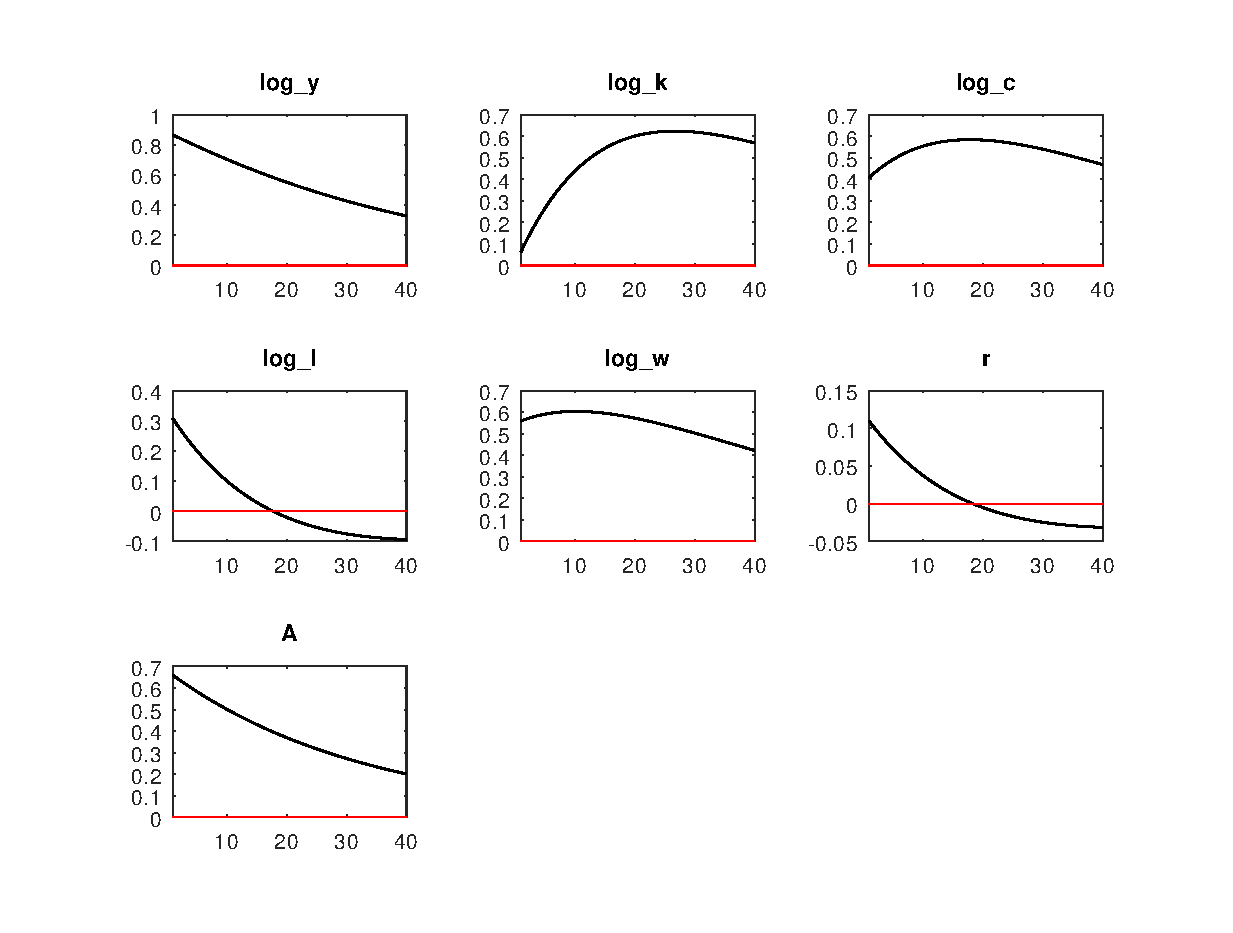
\includegraphics[width=0.80\textwidth]{RBCp_IRF_eps_A}

	\label{fig:rbcefectodynareptfpermanente}
\end{figure}
\renewcommand{\rgcaptioneq}{\rgcaption{Efecto de un shock de oferta permanente en un modelo del ciclo real básico\footnote{Estimado con modelo RBC\_Baseline.mod de \href{https://github.com/JohannesPfeifer/DSGE_mod}{Repositorio de modelos DSGE en Dynare de Johannes Pfeifer.}}.}}
\begin{center}
\rgcaptioneq
\end{center}


\begin{figure}[!htbp]
	\psfrag{log_y}[1][][0.5][0]{${\log(y)}$}
	\psfrag{log_k}[1][][0.5][0]{${\log(k)}$}
	\psfrag{log_c}[1][][0.5][0]{${\log(c)}$}
	\psfrag{log_l}[1][][0.5][0]{${\log(l)}$}
	\psfrag{log_w}[1][][0.5][0]{${\log(w)}$}
	\psfrag{r}[1][][0.5][0]{${r}$}
	\psfrag{A}[1][][0.5][0]{${A}$}
	\centering 
	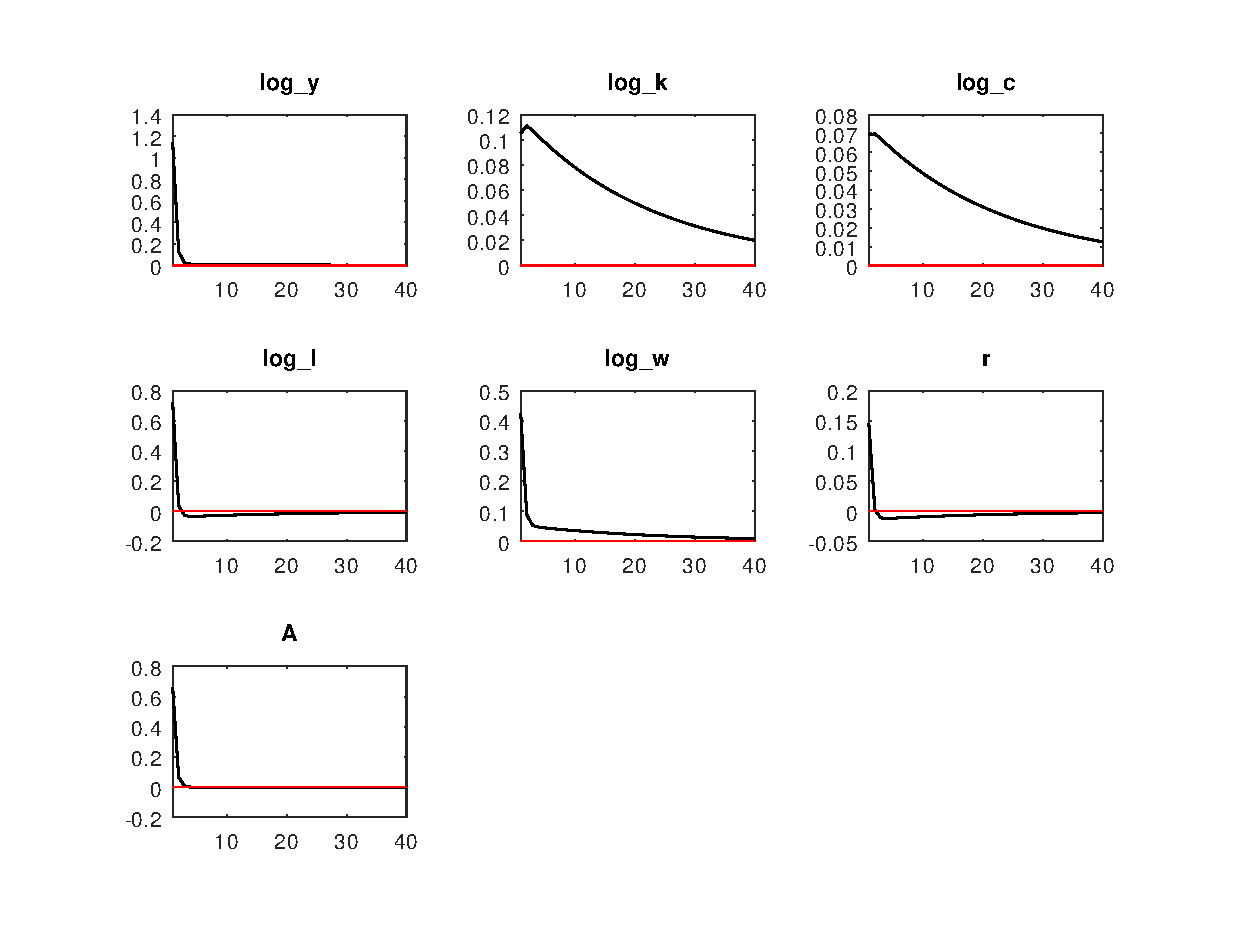
\includegraphics[width=0.80\textwidth]{RBCt_IRF_eps_A}
	
	\label{fig:rbcefectodynareptftransitorio}
\end{figure}
\renewcommand{\rgcaptioneq}{\rgcaption{Efecto de un shock de oferta transitorio en un modelo del ciclo real básico\footnote{Íbidem.}}}
\begin{center}
	\rgcaptioneq
\end{center}



%\pagebreak

%\begin{tabla}{Representación gráfica de los efectos de un shock de oferta positivo en un modelo del ciclo real simple calibrado para la economía americana en las últimas décadas.}{rbcshockprod}
	
%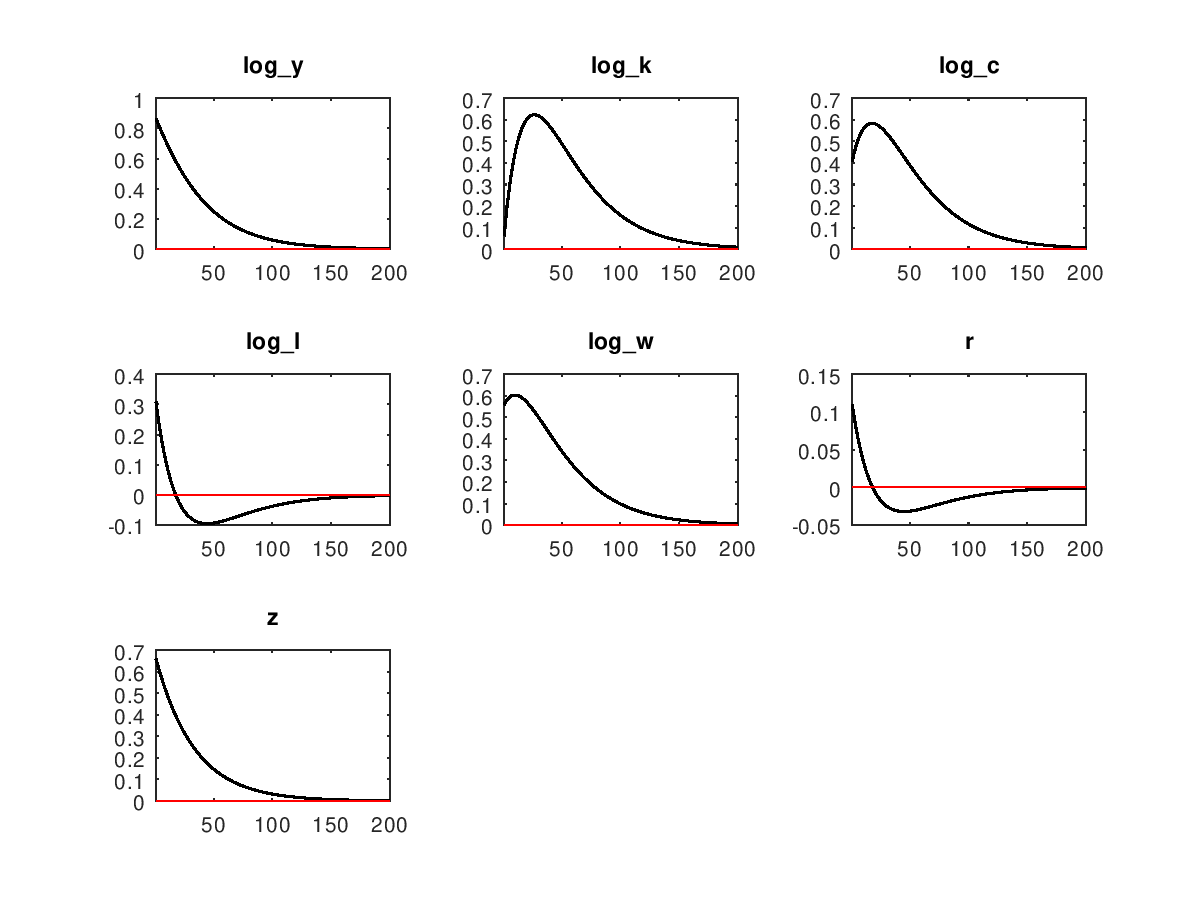
\includegraphics[scale=0.65]{RBC_Baseline_Shock_Productivity.png}
%%%\end{tabla}

%\begin{tabla}{Representación gráfica de los efectos de un shock de oferta positivo en un modelo canónico de la NEK de segunda generación.}{nekshockprod}{}
	
%\includegraphics[scale=0.65]{NEK_Baseline_Shock_productivity.png}
%\end{tabla}


\preguntas



\seccion{Preguntas cante 2016}

\begin{itemize}
    \item Ante una subida del precio del petróleo, ¿qué debe hacer el gobierno? ¿Y ante una bajada?
    \item ¿Cómo puede España reducir la dependencia energética?
    \item En relación a las nuevas tecnologías y los shocks, ¿existe relación entre las TIC y la inflación? ¿y entre las TIC y la competencia?
    \item ¿Por qué la curva renta-tipo de cambio tiene pendiente negativa en el modelo de la NEK que ha cantado?
\end{itemize}

\seccion{Test 2009}

\textbf{13.} Considere el marco teórico y metodológico de los modelos macroeconómicos estáticos. Indique entre las siguientes afirmaciones cuál es la CORRECTA:

\begin{itemize}
	\item[a] Si los precios y los salarios son flexibles, un shock positivo de la productividad total de los factores incrementa el consumo y la inversión, pero no afecta el empleo.
	\item[b] Si el salario real es rígido y constante, y los precios son rígidos, un shock positivo de la productividad total de los factores incrementa el paro total, aumentando el paro keynesiano y disminuyendo el paro clásico.
	\item[c] Si los precios son flexibles y el salario nominal es rígido, un shock positivo de la productividad total de los factores afecta negativamente al consumo, a la inversión y al empleo.
	\item[d] Si el salario real es rígido y constante, y los precios son rígidos,un shock positivo de la productividad total de los factores no altera el nivel de paro, aunque sí la composición entre paro keynesiano y paro clásico.
\end{itemize}

\seccion{Test 2005}

\textbf{13.} Suponga una economía con una tecnología agregada de producción del tipo Cobb-Douglas: $Y=F(K,L) = \theta K^{\alpha_1} L^{\alpha_2}$, $\alpha_1 + \alpha_2 \leq 1$, $\theta$: perturbación de oferta. Si se observa un incremento del empleo, éste podría deberse a:

\begin{itemize}
	\item[a] Un incremento en el coste de uso del capital.
	\item[b] Un aumento en el grado de competencia de los mercados de bienes.
	\item[c] Los empresarios se volvieron más aversos al riesgo.
	\item[d] Una perturbación negativa de oferta.
\end{itemize}

\notas

\textbf{2009} \textbf{13.} B

\textbf{2005} \textbf{13.} B

El artículo de Ball y Mankiw (2002) referenciado en la bibliografía de este tema y del 3B-31 se refiere al intento de modelizar una teoría de los \comillas{supply shocks} en Ball and Mankiw (1995).

\bibliografia

\begin{itemize}
	\item cost-push inflation
	\item energy-GDP relationship
	\item energy price shocks
	\item ICT, internet and worker productivity
	\item oil and the macroeconomy
	\item supply shocks in macroeconomics
\end{itemize}

Acemoglu, D.; Ozdaglar, A.; Tahbaz-Salehi, A. (2017) \textit{Microeconomic Origins of Macroeconomic Tail Risks} American Economic Review -- En carpeta del tema

Ball, Mankiw (2002) \textit{The NAIRU in theory and practice.} Journal of Economic Perspectives

Ball, Mankiw (1995) \textit{Relative-price changes as aggregate supply shocks.} Quarterly Journal of Economics

Baqaee, D. R.; Farhi, E; \textit{The Macroeconomic Impact of Microeconomic
Shocks: Beyond Hulten’s Theorem} \url{https://scholar.harvard.edu/files/farhi/files/beyond_hulten_draft.pdf}

Bernanke, B. S.; Gertler, M.; Watson, M. (1997) \textit{Systematic Monetary Policy and the Effects of Oil Price Shocks} Brookings Papers on Economic Activity -- En carpeta del tema

\textbf{Blanchard, O. J.; Galí, J. (2008) \textit{The Macroeconomic Effects of Oil Price Shocks: Why are the 2000s so different from the 1970s?} MIT Working Paper Series -- En carpeta del tema}

Blinder, A. S.; Rudd, J. B. (2013) \textit{The Supply-Shock Explanation of the Great Stagflation Revisited} En ``The Great Inflation: The Rebirth of Modern Central Banking'' -- En carpeta del tema

Boeh, C.; Flaaen, A.; Pandalai-Nayar, N. (2015) \textit{The role of global supply chains in the transmission of shocks: Firm-level evidence from the 2011 Tohoku earthquake} VoxEU -- \url{https://voxeu.org/article/global-supply-chains-and-transmission-shocks}

\textbf{Carvalho, V. M. (2014) \textit{From Micro to Macro via Production Networks} Journal of Economic Perspectives. Volume 28, Number 4 - Fall 2014 -- En carpeta del tema}

Carvalho, V. M.; Nirei, M.; Saito, Y. U.; Tahbaz-Salehi, A. (2016) \textit{Supply Chain Disruptions: Evidence from the Great East Japan Earthquake} Cambridge-INET Working Paper Series No: 2016/25 -- En carpeta del tema

De Grauwe, P. (2014) \textit{Yes, it's the economy, stupid, but is it demand or supply?} CEPS Commentary -- En carpeta del tema

Galí, J.; López-Salido, J. D.; Vallés, J. (2002) \textit{Technology Shocks and Monetary Policy: Assessing the Fed's Performance} NBER Working Papers -- En carpeta del tema

\textbf{Garganas, N. (2006) \textit{Macroeconomic management in an environment of aggregate supply shocks -- lessons from recent experience} Background paper to speech, at the SEANZA Symposium -- En carpeta del tema}

Gramlich, E. M. (1979) \textit{Macro Policy Responses to Price Shocks} Brookings Institution -- En carpeta del tema

Hamilton, J. D. (2000) \textit{What is an Oil Shock} NBER Working Paper Series -- En carpeta del tema

Hamilton, J. D. (2009) \textit{Causes and Consequences of the Oil Shock of 2007-08} NBER Working Paper Series -- En carpeta del tema

Hamilton, J. D.; Herrera, A. M. (2000) \textit{Oil Shocks and Aggregate Macroeconomic Behavior: The Role of Monetary Policy} 

Inoue, H.; Todo, Y. (2019) \textit{Propagation of economic shocks through supply chains} VoxEU -- \url{https://voxeu.org/article/propagation-economic-shocks-through-supply-chains}

Kilian, L.. (2006) \textit{Not All Oil Price Shocks are Alike: Disentangling Demand and Supply Shocks in the Crude Oil Market} American Economic Review. Vol. 99. No. 3 June 2009 -- En carpeta del tema

\textbf{Kilian, L. (2008) \textit{The Economic Effects of Energy Price Shocks} Journal of Economic Literature -- En carpeta del tema}

Pfeifer, J. \textit{DSGE\_Mod: A collection of Dynare Models} \url{https://github.com/JohannesPfeifer/DSGE_mod}

Ramey, V. A. (2016) \textit{Macroeconomic shocks and their propagation}  NBER Working Paper Series -- En carpeta del tema

Ramey, V. A. \textit{Chapter 2. Macroeconomic Shocks and Their Propagation} Handbook of Macroeconomics 2 -- En carpeta Libros/Macro

\textbf{Shapiro, M. (1987) \textit{Supply Shocks in Macroeconomics} Cowles Foundation Discussion Paper No. 821 -- En carpeta del tema}

Wieland, J. (2017) \textit{Are Negative Supply Shocks Expansionary at the Zero Lower Bound} 

\end{document}
